\documentclass{beamer}
%\usetheme{Malmoe}
\usefonttheme{structuresmallcapsserif}
\usecolortheme{beaver}
\usepackage[ngerman, main=english]{babel}
\usepackage{fontspec}
\usepackage{amsmath}
\beamertemplatenavigationsymbolsempty
\setbeamertemplate{caption}{\raggedright\insertcaption\par}

%\usepackage{csquotes}
%\usepackage{amssymb}
\usepackage{float}
%\usepackage{hyperref}
\usepackage{cleveref}
\usepackage{nicefrac}
\include{jkcommands}

%\usepackage{mathpazo}
\setsansfont[Numbers=OldStyle]{Linux Libertine O}
%\setkomafont{sectioning}{\scshape}

\title{Ac-Stark shift of Lithium-6 in an Optical Dipole Trap}
\author{Jonathan Förste}
\date{\today}

\begin{document}

\maketitle
\begin{frame}
	\frametitle{Motivation}
	\begin{figure}
	\centering
	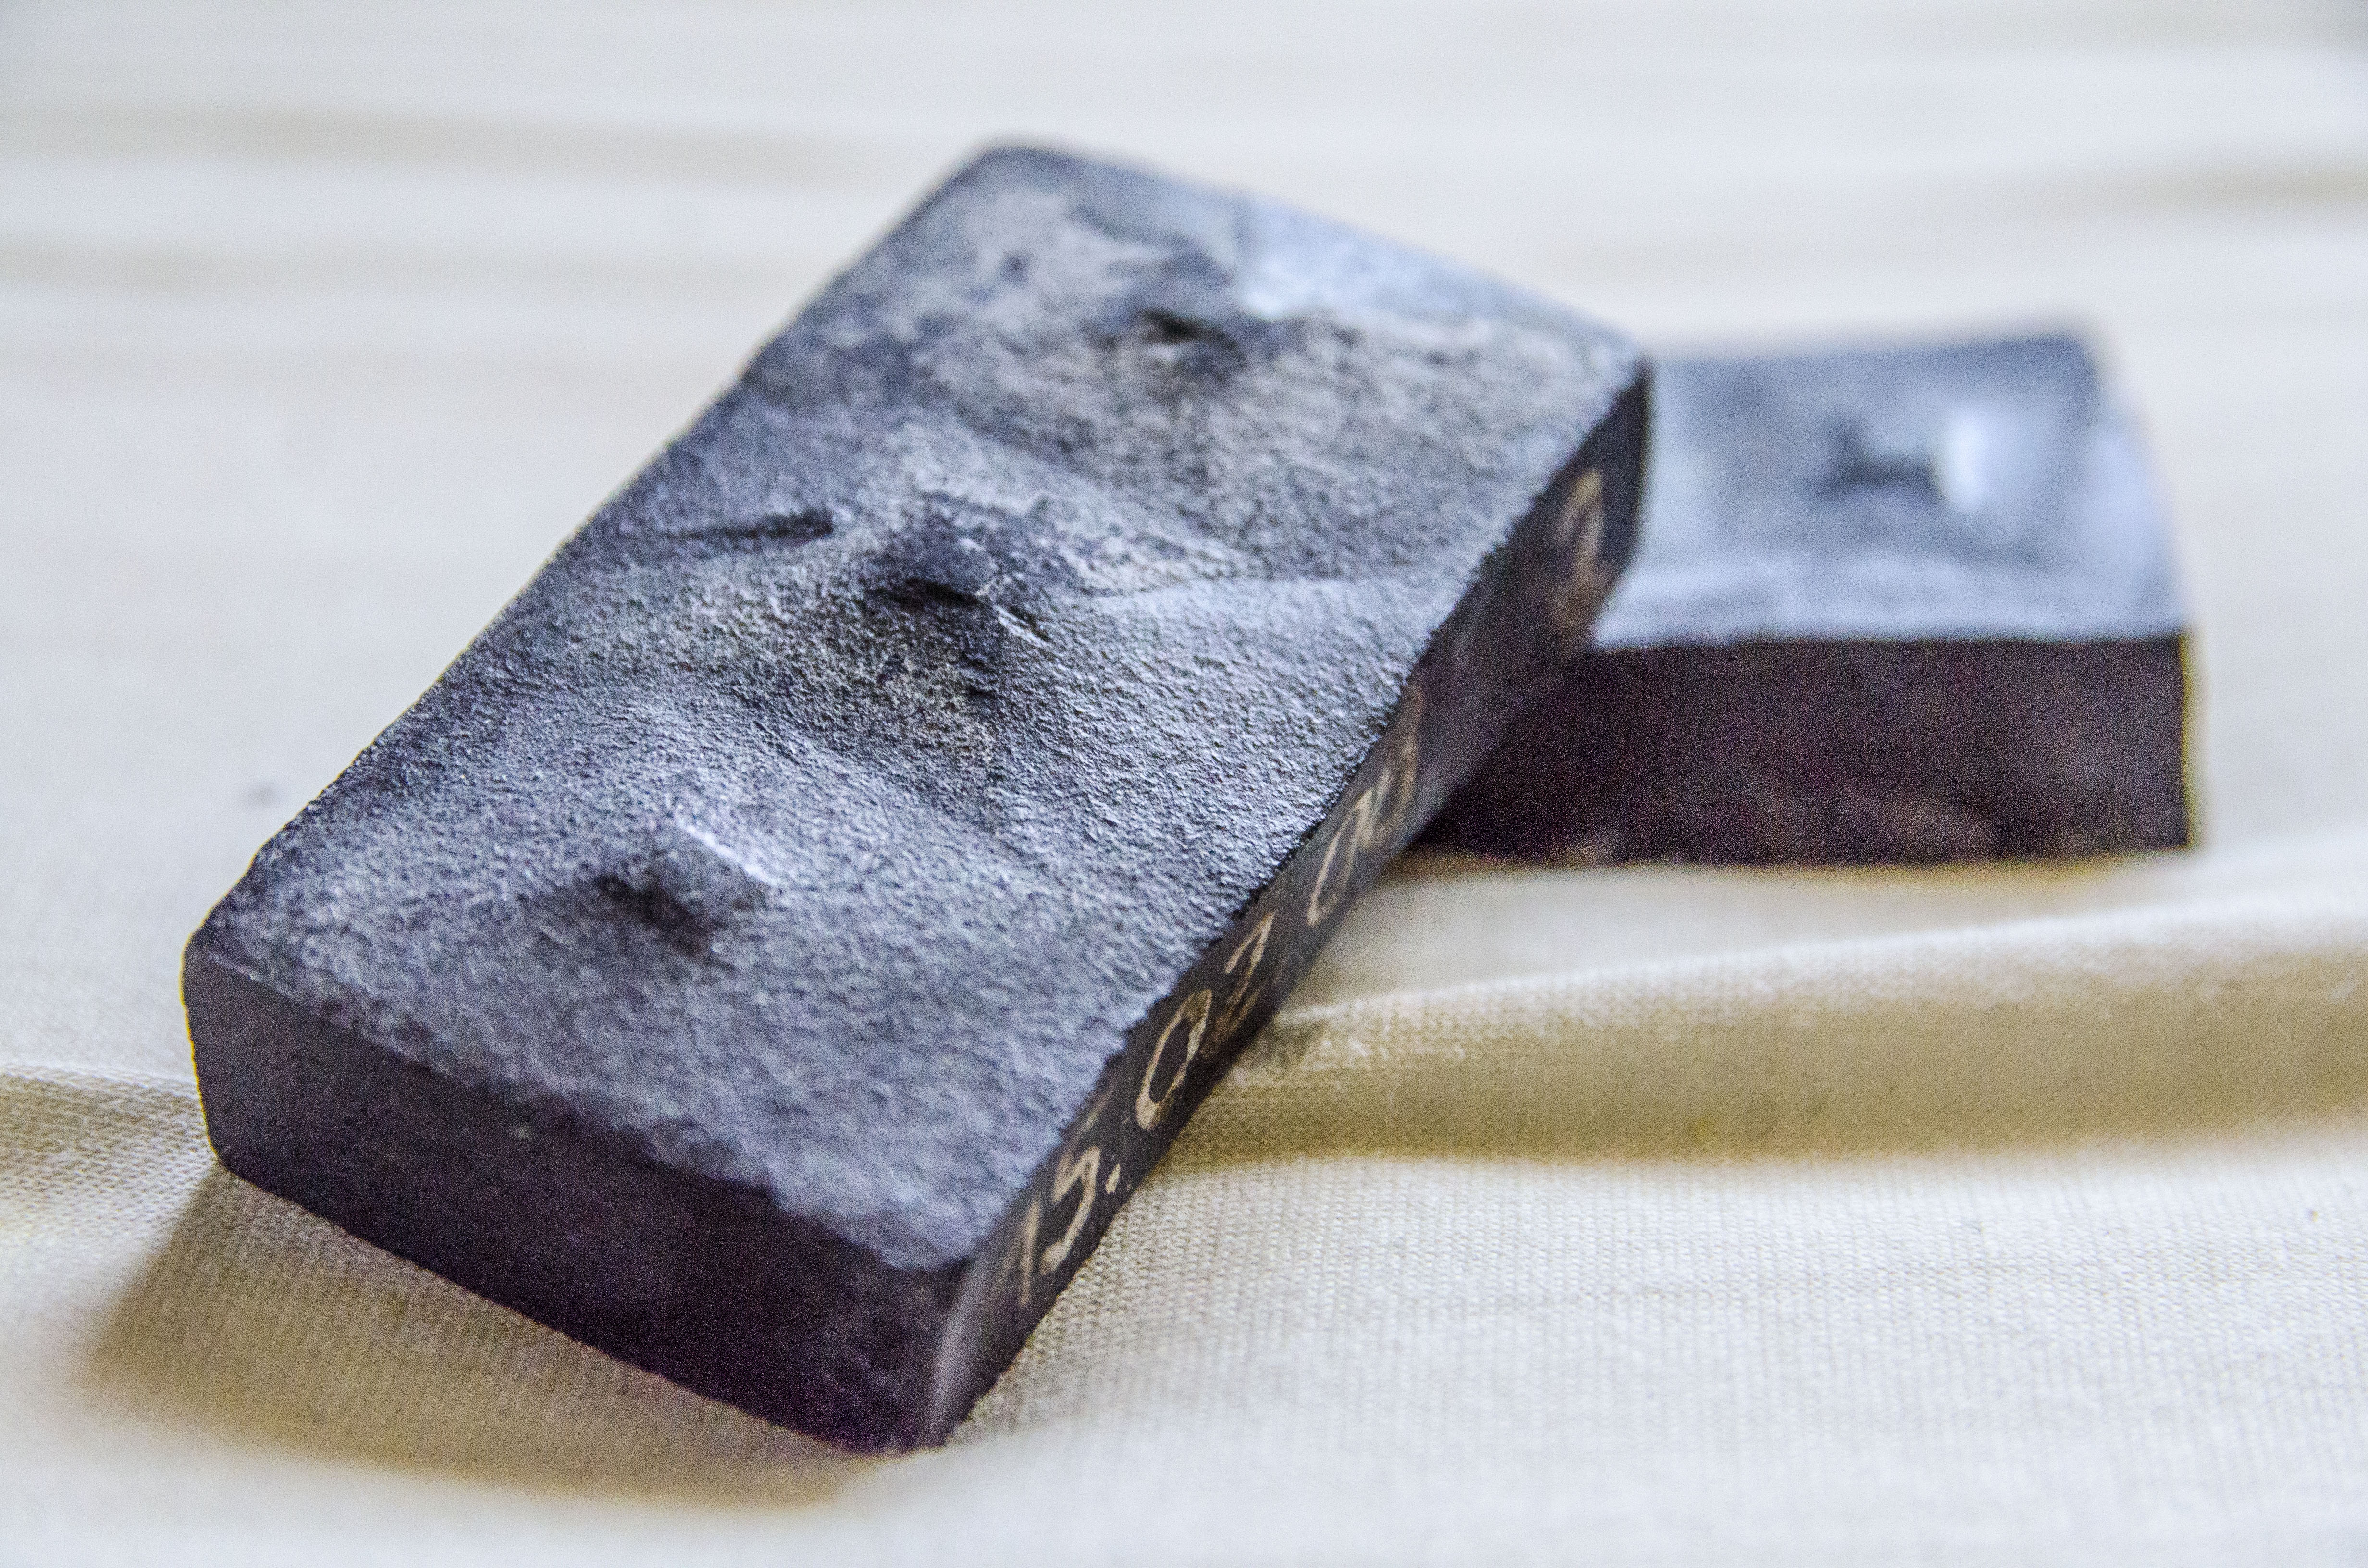
\includegraphics[scale=0.06]{supraleiter_1}
	\caption{Hochtemperatur-Supraleiter}
	\end{figure}
\end{frame}

%\begin{frame}
%	\frametitle{Motivation}
%	\begin{figure}
%	\centering
%	\includegraphics[scale=0.4]{lattice}
%	\caption{Optisches Gitter}
%	\end{figure}
%	
%\end{frame}
%\begin{frame}
%	\frametitle{Motivation}
%	\begin{figure}
%	\centering
%	\includegraphics[scale=0.6]{spilling}
%	\caption{Präparation weniger Atome}
%	\end{figure}
%\end{frame}

\begin{frame}
	\frametitle{Motivation}
	\begin{figure}
	\centering
	\includegraphics[scale=0.7]{potentials}
	\caption{Doppeltopf-Potential}
	\end{figure}
\end{frame}
\begin{frame}
	\frametitle{Motivation}
	\begin{figure}
	\centering
	\includegraphics[scale=0.7]{octagon}
	\caption{Aufbau des Experiments}
	\end{figure}
\end{frame}
\begin{frame}
	\frametitle{Motivation}
	\begin{figure}
	\centering
	\includegraphics[scale=0.22]{newscheme}
	\caption{Schema für neues Imaging}
	\end{figure}
\end{frame}
\begin{frame}
	\frametitle{Theorie und Berechnung}
	\begin{figure}
	\centering
	\includegraphics[scale=0.22]{feder}
	\caption{Klassisches Bild}
	\end{figure}
\end{frame}
\begin{frame}
	\frametitle{Theorie und Berechnung}
	\begin{figure}
	\centering
	\includegraphics[scale=0.4]{classicpotential}
	\caption{Klassisches Dipol-Potential}
	\end{figure}
\end{frame}
\begin{frame}
	\frametitle{Theorie und Berechnung}
\begin{center}
	\begin{figure}
                \includegraphics[scale=0.22]{levels2}
           	\caption{Termschema von Lithium}
\end{figure}
\end{center}
\end{frame}
\begin{frame}
	\frametitle{Theorie und Berechnung}
\begin{center}
	\begin{figure}
                \includegraphics[scale=0.24]{polarizegr}
           	\caption{Polarisierbarkeit des Zustandes $2s_{1/2}$}
\end{figure}
\end{center}
\end{frame}
\begin{frame}
	\frametitle{Theorie und Berechnung}
\begin{center}
	\begin{figure}
                \includegraphics[scale=0.24]{polarizeex1}
           	\caption{Polarisierbarkeit des Zustandes $2p_{3/2}, |m_J|=1/2$ }
\end{figure}
\end{center}
\end{frame}
\begin{frame}
	\frametitle{Theorie und Berechnung}
\begin{center}
	\begin{figure}
                \includegraphics[scale=0.24]{polarizeex2}
           	\caption{Polarisierbarkeit des Zustandes $2p_{3/2}, |m_J|=3/2$}
\end{figure}
\end{center}
\end{frame}
\begin{frame}
	\frametitle{Theorie und Berechnung}
\begin{center}
	\begin{figure}
                \includegraphics[scale=0.7]{alphaalltogether}
           	\caption{Polarisierbarkeiten der Zustände $2s_{1/2}$ (Rot), $2p_{3/2}, |m_J|=1/2$ (Blau), $2p_{3/2}, |m_J|=3/2$ (Gelb) }
\end{figure}
\end{center}
\end{frame}
\begin{frame}
	\frametitle{Messung}
\centering
	\begin{figure}
                \includegraphics[scale=0.4]{dipolefoto}
           	\caption{Absorbtionsbild der gekreuzten Dipolfalle}
\end{figure}
\end{frame}
\begin{frame}
	\frametitle{Messung}
\centering
	\begin{figure}
                \includegraphics[scale=0.22]{withwithout}
           	\caption{Beispiel für Resonanzverschiebung der $D_2$-Linie}
\end{figure}
\end{frame}
\begin{frame}
	\frametitle{Messung}
\centering
	\begin{figure}
                \includegraphics[scale=0.3]{shiftintens-eps-converted-to}
           	\caption{Resonanzverschiebung $D_2$-Linie}
\end{figure}
\end{frame}
\end{document}